\chapter{Magic}
\label{ch:magic}

This discipline represents common magic or hedge magic. It is the typical type of magic that most campaigns will have. Magic is generally of a practical nature, meant to address battle or the common ills of the community: healing the sick, bringing love or luck, driving away evil forces, finding lost items, reading omens and so on. 


\section{Spot Rules}

\subsection{Learning Magic}
Magic Casting is treated as a skill. The base chance for Magic Casting is POWx3. Spells are learnt separately, but the Magic Casting skill determines the success for casting all Magic spells. Characters learn Magic from other characters who know the practice. It costs four Improvement Points to get access to the Magic discipline.

\subsection{Learning Spells}
Characters learn Magic spells from other characters who know the appropriate spells. Learning spells costs one Improvement Point per Magnitude point. If a character knows a spell at a lower Magnitude, they only have to pay the difference in Improvement Points to gain the spell at a higher Magnitude.

\begin{rpg-examplebox}
Adjin already knows Coordination at 2 Magnitude. He wants to learn Coordination 3, so he must only spend one Improvement Point to gain the spell at that Magnitude.
\end{rpg-examplebox}

A character has a limit of their POWx2 in magnitude in spells. So a character with a POW of 10 can learn s AAAA

Magic can be learnt from a number of sources. The most typical is from some kind of school of magic appropriate for the campaign or from remote hermits and otherworldly Shamans who commune with the Spirit World and learn it's secrets. In some cases, it can be learnt from local priests who teach Magic associated with their gods’ mythological exploits.

In each case the player character must be in good standing with the teacher before they will teach them the spell. If the teacher is indifferent to the player character to start with then they will first need to undertake some kind of service, which can be the focus of an adventure.

\subsection{Casting Spells}
A character must be able to move his hands to make gestures, be able to chant and be able to see his target in order to cast a spell.

When the character is casting a spell under duress, such as in the midst of combat, they must pass a Magic Casting test to successfully cast the spell. In this regard Magic is like any other skill. If the character is relaxed and has all the time in the world then no casting test is needed, the spell is automatically cast.

The result of the Magic casting test depends on its success:
\begin{description}
	\item[Success:] A number of Power Points are deducted from the spellcaster’s total, equal to the Magnitude of the spell. The spell then takes effect.
	\item[Failure:] The spell does not take effect and the character loses one Power Point.
	\item[Critical:] The caster has been able to control the flow of the magic particularly effectively. The character loses one Power Point instead of the normal cost of the spell.
	\item[Fumble:] The caster has been unable to control the flow of the Magic. Rather than losing a single Power Point for failing to cast the spell, the caster loses a number of Power Points equal to its Magnitude. 
\end{description}

\begin{figure}[h]
\begin{center}
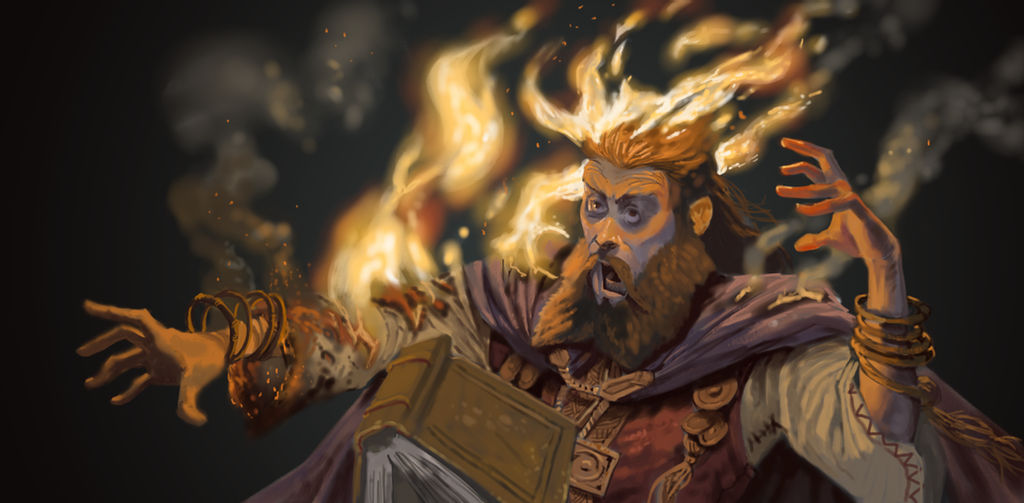
\includegraphics[scale=0.23]{img/backfire_by_ncorva.jpg}
\end{center}
\end{figure}


\subsubsection{Casting Time}
No other action may be taken whilst casting a spell, though the character may slowly walk up to half their Movement while spell casting. %All spells take one combat round to cast.

Casting begins at the start of the combat round and a spell’s effect happens on the caster’s Combat Order.% INT, instead of DEX, (which is used for close combat).  

Distractions, or attacks on the caster as he casts, will automatically ruin the spell, unless the caster successfully passes a Persistence test, thereby maintaining concentration on the spell. Examples of distraction include blinding, disarming, or wounding the caster.

\subsubsection{Dismissing Spells}
In a single Combat Round, a caster can dismiss any Permanent spell(s) he has cast, as a free action. Ceasing to cast a Concentration spell is immediate and not an action. 


\subsection{Spell Traits}
Unless otherwise stated all Magic spells have the following traits.

\begin{rpg-list}
\item They have Variable Magnitude. This means that the Magnitude of the spell starts from the stated Magnitude and then can be cast at a higher Magnitude, if the caster knows it, giving an increase in the effect of the spell. The maximum Magnitude that a caster can learn is equal to their POW divided by 3.
\item The Base Magnitude is one. 
\item Range is equal to the caster’s POWx3 in metres.
\item They have a Duration of ten minutes.
\end{rpg-list}

Other traits used by spells are detailed below. 
\begin{description}
	\item[Area (X):] The spell affects all targets within a radius specified in metres. 
	\item[Concentration:] The spell’s effects will remain in place so long as the character continues to concentrate on it. Concentrating on a spell is functionally identical to casting the spell, requiring the caster to continue to chant and ignore distractions. 
	\item[Instant:] The spell’s effects take place instantly. The spell itself then disappears. 
	\item[Magnitude (X):] The strength and power of the spell. Also the minimum number of Power Points required to cast it. 
	\item[Non-Variable:] The spell may only be cast at the stated Magnitude.
	\item[Permanent:] The spell’s effects remain in place until they are dispelled or dismissed. 
	\item[Resist (Dodge/Persistence/Resilience):] The spell’s intended effects do not succeed automatically. The target may make a Dodge, Persistence or Resilience test (as specified by the spell) in order to avoid the effect of the spell entirely. Note that Resist (Dodge) spells require the target to be able to use Reactions in order to Dodge. In the case of Area spells, the Resist (Dodge) trait requires the target to dive in order to mitigate the spell’s effect. 
	\item[Touch:] Touch spells require the character to actually touch his target for the spell to take effect, using a Unarmed skill test to make contact. The caster must remain in physical contact with the target for the entire casting.
	\item[Trigger:] The spell will lie dormant until an event stated in the description takes place. The spell then takes effect and is expended.
\end{description}

\section{Spells}


\begin{rpg-spell}
{Animal Whisperer}
{Magnitude 2, Non-Variable, Touch}

The caster whispers into the ear of a distressed animal, calming it. If the distressed animal is under the influence of a spell such as Fear or Scare, then its gets another Persistence test to shake off the effect of the spell.
\end{rpg-spell}


%\begin{rpg-spell}
%{Avoidance}
%{Instant, Trigger}
%
%This spell lies dormant until the recipient is attacked. Then, after the normal reaction of the recipient, it fires off allowing the recipient to Dodge a number of times equal to the spell’s Magnitude. Once triggered, all the extra Dodge reactions are valid for that round only.
%\end{rpg-spell}


\begin{rpg-spell}
{Babel}
{Magnitude 2, Non-Variable, Resist (Persistence)}

If this spell is successful, it garbles the language of the affected creature. The target can still think and, for the most part, act normally, but anything it says comes out as gibberish. Thus, a commanding officer would be unable to give orders to his men and a spellcaster would be unable to cast spells.
\end{rpg-spell}



\begin{rpg-spell}
{Back Eyes}
{Magnitude 2, Non-Variable}

This spell grants the recipient awareness as if they had physically got eyes in the back of their head for the duration of the spell, which allows them to make Perception rolls and be aware of others behind them.
\end{rpg-spell}


% TO DELETE - covered by Enhance Skill !!
%\begin{rpg-spell}
%{Bearing Witness}
%{Instant}
%
%This spell grants the caster a +10\% bonus per point of Magnitude to their next Skill Test they make to discover lies, secrets or hidden objects. It does not stack with any other spell-effect bonuses.
%\end{rpg-spell}


\begin{rpg-spell}
{Beast Call}
{Magnitude 2, Non-Variable, Instant, Resist (Resilience)}

The Beast Call serves to attract an animal within range. When the spell is cast, it affects a targeted creature with a fixed INT of 7 or less. If it fails to resist, the creature will be naturally drawn to the place where the spell is cast, whereupon the spell effect terminates. Any barrier, immediate threat, or counter control, also ends the effects of the spell, leaving the creature to react naturally. 

For example, the Beast Call spell might cause a horse to turn and walk towards the spell, but a single yank of its reins by the rider would end the spell’s effect. This spell is a potent aid to hunters and herders.
\end{rpg-spell}


\begin{figure*}
\begin{center}

\includegraphics[scale=2.1]{img/mystical_forest_by_sirend.jpg}
\end{center}
\end{figure*}


\begin{rpg-spell}
{Befuddle}
{Magnitude 2, Non-Variable, Resist (Persistence)}

This spell confuses and clouds the mind of its target if they fail a Persistence roll. The affected target may not cast spells and may only take non-offensive actions. The target may run if it so chooses and may dodge and normally parry in combat. Any skills that have INT as a base are at -20\% when tested while the target is under the effects of this spell.

This spell is effective against humanoids and natural creatures. Other creatures (such as spirits or magical beasts like dragons) are not affected by this spell.
\end{rpg-spell}


\begin{rpg-spell}
{Block Sense}
{Magnitude 3, Non-Variable, Resist (Persistence)}

Depending on the version of this spell it will Blind/Deafen/Desensitise taste or smell/Numb touch on a failed resistance roll for the duration of the spell.
\end{rpg-spell}


\begin{rpg-spell}
{Call Spirit (Type)}
{Magnitude 3, Non-Variable, Resist (Persistence)}

This spell summons a single spirit of a given type from the Spirit World to do the bidding of the caster. The spirit resists the call by using its Persistence. If it succeeds, it can return to the Spirit World. Unless combined with a Binding attempt (see below), the spirit that fails a Persistence roll must perform one action, within its power, for the caster, after which it returns to the Spirit World.

\begin{rpg-list}
\item Disease spirits, inflict disease upon the possessed victim.
\item Passion (Fear/Madness/Pain) these spirits work upon the passions of a victim and cause mental debilitation and distress.
\item Healing spirits, can be used to heal wounds and drive out possessing Disease spirits.
\item Magic spirits, know spells and have power points that the caller may use.
\item Guardian Spirits, protect a location for the casters POW in minutes.
\item Ancestor Spirit, can pass on one piece of wisdom or increase one skill for the spell's duration.
\end{rpg-list}
\end{rpg-spell}

 
\begin{rpg-spell}
{Care}
{Magnitude 2, Non-Variable, Touch}

This charm places the recipient under the care of the caster. If the caster has any active Protection or Countermagic spells, the Cared for character also benefits from the effects of these spells.
\end{rpg-spell}

\begin{rpg-spell}
{Clear Path}
{Touch}

This spell allows the caster to move through even the most tangled, thorny brush, as if they were on an open road. For each additional point of Magnitude, they may bring one person with him. 
\end{rpg-spell}


\begin{rpg-spell}
{Coordination}
{Touch}

For every point of Magnitude, the target’s combat order increases by +2, whether casting spells or fighting and 10\% is added to Dodge or DEX-based Athletics tests. 
\end{rpg-spell}


\begin{rpg-spell}
{Counter-Attack}
{Magnitude 2, Non-Variable, Trigger}

This spell lies dormant until the recipient is attacked. Then, after the normal defensive reaction of the recipient, it fires off, allowing the recipient to follow up with a counter attack. The counter attack is an additional action, on top of the recipient’s normal attacking action.
\end{rpg-spell}


\begin{rpg-spell}
{Counter-Defense}
{Magnitude 2, Non-Variable, Trigger}

This spell lies dormant until the recipient is successfully attacked. Then after the normal reaction of the recipient, it fires off allowing the recipient an extra defence.
\end{rpg-spell}



\begin{rpg-spell}
{Countermagic}
{Instant}

Countermagic is only ever used as a Reaction, and only when another spell is cast within Countermagic’s Range that the character wishes to counter. A successful Countermagic disrupts the other spell and nullifies it. As long as Countermagic’s Magnitude equals or exceeds the target spell’s Magnitude, the target spell is countered.
\end{rpg-spell}


\begin{rpg-spell}
{Cover Blind Side}
{Magnitude 1, Non-Variable}

For the duration of the spell, the target can react to attacks from behind or flank attacks as if they were a normal attack from the front. It does not confer any additional reactions.
\end{rpg-spell}


\begin{rpg-spell}
{Create Charms}
{Permanent}

A charm is a physical item that stores one or more Magic spells. A charm could be a necklace that holds a Befuddle 4 spell, a shield etched with runes that holds a Countermagic 2 spell, or even a sheet of paper with a poem written on it that, when held against the skin, provides a Protection 1 spell.

\begin{rpg-list}
\item To create a charm a character must possess both the spell they wish to store and Create Charm at the same Magnitude.
\item The item into which the charm is to be cast must be prepared and in contact with the caster for the length of the casting.
\item If the caster spends one Improvement Point at the time of creation, the spell is reusable. Otherwise once the spell is cast the Charm is dispelled. A spell stored in a Charm is used like any other spell that the possessor knows. It uses the wielder’s Magic Casting skill and is powered by the wielder’s Power Points.
\item If the caster spends three Improvement Points per Magnitude at the time of creation the spell within the Charm is reusable, once per day (1/day), without requiring a Magic Casting skill or any Power. It can be activated as an Action. If the Create Charms spell is cast again then it becomes 2/day, and so on. Not all spells can be stored this way and the Gamemaster has the final say.
\item If the caster spends ten Improvement Points per Magnitude at the time of creation the spell within the Charm is always active, without requiring a Magic Casting skill or any Power. These are the most powerful charms. Not all spells can be stored this way and the Gamemaster has the final say.
\item The time taken to create a single-use Charm is one hour per point of Magnitude of the spell being stored; Reusable Charms take three hours per point of Magnitude to create.
\item Charms are mundane items. Breaking the item dispels the Charm.
\end{rpg-list}
\end{rpg-spell}


\begin{rpg-spell}
{Create Power Point Store}
{Permanent}

This spell allows the caster to create an item which has Power Point storing capabilities. This allows the owner to have a pool of Power Points in addition to their own.

Typically crystals are used, due to their physical toughness, in game terms treat them as unbreakable. This also applies to charms, such as a sword with Weapon Enhancement 2 stored in it, to provide a pool of power points to cast the spell from.

Power Point stores take one hour per Power Point stored in them to create. For each Magnitude, one Power Point can be stored.

Unless one Improvement Point is spent when they are created they are non-reusable. Once the Power Points are used the item loses its ability to store Power Points. If the Improvement Point is spent the item then becomes reusable. Once all the Power Points are used, the item can be refilled instantly from the user’s own Power Points.

The caster must fill the item with their own Power Points as part of the spell. The amount of Power Points put into the item at the time of casting becomes the maximum that can be put into the item. This maximum can not be increased after the spell is cast.

If the item is damaged or destroyed the Power Points are released harmlessly into the surrounding area.
\end{rpg-spell}

% TODO check all spells here and compare/contrast with OQ3 SRD, OQ2 hard cover, etc.

\begin{rpg-spell}
{Create Potions}
{Permanent}

Potions are liquids that store one or more Magic spells. The Magnitude of the Create Potion spell needs to equal or exceed the highest Magnitude of the spell being stored into the potion.

\begin{rpg-list}
\item All potions are one use. They must be drunk in one swift gulp to work. 
\item The potion automatically works and doesn’t incur a cost in Power Points to the person who is drinking it. 
\item If multiple spells are placed in the potion, they are all cast on the drinker when the potion is drunk.
\item The potion costs the enchanter Power Points. They must know the spell at the Magnitude enchanting at, with the Power Points of the spell(s) placed into the potion. 
\item There is an associated cost of 10 Gold Pieces per Magnitude in materials, which includes the flask that contains the potion. 
\item To make the potion, the enchanter must roll successfully against Magic Casting for each spell being placed in the potion and against Lore (Potion Making). If they fail the potion is ruined and they lose the cost of the ingredients. 
\item Potions take one hour per point of Magnitude of spell(s) stored to create. 
\item A potion must be stored in an airtight container, or it evaporates, losing one point of Magnitude per week. 
\end{rpg-list}
\end{rpg-spell}



\begin{rpg-spell}
{Create Scrolls}
{Permanent}

This spell allows the caster to create a written version of the spell for later use. Either to impart knowledge of the spell to a trainee or as a reference when casting the spell in the field.

\begin{rpg-list}
\item The caster must be able to read and write in some form of written language, which is represented by having a Language skill of over 80\%. They must also pay for the special inks and scroll paper (10 Gold Pieces per point of magnitude).
\item The trainee must be able to read the language that the scroll uses. Once every three months they may study the scroll, which takes one day per point of spell, and then make a Language skill test. If successful, they spend the normal Improvement Point cost to learn the spell. If they roll a critical they spend half that cost, to the nearest whole unit. If they fumble, they can never learn the spell from that scroll, it is beyond their understanding.
\item To directly cast a spell from the scroll, the caster must be able to read the language the scroll uses. Then cast the spell as normal. Casting is much slower than if the caster is casting the spell from memory. First, the caster reads the spell out loud and then harnesses and shapes the magical energies. Therefore, no matter what their normal casting skill, the spell takes an entire combat round to cast, and fires off at the end of the combat round.
\end{rpg-list}
\end{rpg-spell}


\begin{rpg-spell}
{Cushion Fall}
{Magnitude 2, Non-Variable}

The successful casting of the spell eliminates all falling damange for the recipient for the duration of the spell.
\end{rpg-spell}


\begin{rpg-spell}
{Darkwall}
{Area 5, Magnitude 2, Non-Variable, Concentration}

Light sources within a Darkwall area shed no light and normal sight ceases to function. Other senses such as a bat’s sonar function normally. 
The caster may move the Darkwall 15 metres per Combat Round if they concentrate on the spell.
\end{rpg-spell}


\begin{rpg-spell}
{Demoralise}
{Magnitude 2, Non-Variable, Resist (Persistence)}

This spell creates doubt and uncertainty into the very heart and soul of the target. The target of this spell has all Weapon skills halved and may not cast offensive spells. If this spell takes effect before combat begins, the target will try to avoid fighting and will either run or surrender. The effects of this spell are automatically cancelled by the Fanaticism spell and vice versa. 
\end{rpg-spell}


\begin{rpg-spell}
{Detext (X)}
{Magnitude 1, Non-Variable, Concentration}

This covers a family of spells that all operate in a similar fashion, allowing the caster to locate the closest target of the spell within its range. This effect is stopped by a thick substance, such as metal, earth or stone, if it is at least one metre thick. It is also blocked by Countermagic, though the caster will know the target is somewhere within range (though not its precise location) and that it is being protected by Countermagic. The separate Detect spells are listed below and each must be learned separately.

\begin{rpg-list}
\item Detect Enemy: Gives the location of the nearest creatures, that intend to harm the caster. 
\item Detect Magic: Gives the location of the nearest magic item, magical creature or active spell. 
\item Detect Species: Each Detect Species spell will give the location of the nearest creature of the specified species. Examples of this spell include Detect Goblin, Detect Rhino and Detect Elf. 
\item Detect Substance: Each Detect Substance spell will give the location of the nearest substance of the specified type. Examples of this spell include Detect Coal, Detect Gold and Detect Wood. 
\end{rpg-list}
\end{rpg-spell}


\begin{rpg-spell}
{Dispel Magic}
{Instant}

This spell will attack and eliminate other spells. Dispel Magic will eliminate a combined Magnitude of spells equal to its own Magnitude, starting with the most powerful affecting the target. If it fails to eliminate any spell (because the spell’s Magnitude is too high), then its effects immediately end and no more spells will be eliminated. A spell cannot be partially eliminated, so a target under the effects of a spell whose Magnitude is higher than that of Dispel Magic will not have any spells currently affecting it eliminated. 
\end{rpg-spell}


\begin{rpg-spell}
{Disruption}
{Instant, Resist (Resilience)}

Disruption literally pulls a target’s body apart. The target will suffer 1D4 points of damage per point of Magnitude, ignoring any Armour Points. 
\end{rpg-spell}


\begin{rpg-spell}
{Dragon Fire}
{Magnitude 2, Non-Variable, Instant, Resist (Dodge)}

With this spell, the caster throws a stream of fire at his target. If the fire is not dodged, it inflicts 1D10 points of heat damage. Armour Points are effective against this damage and it counts as both magical and fire damage.
\end{rpg-spell}


\begin{rpg-spell}
{Drive Out Spirit}
{Instant, Resist (Persistence)}

This spell excommunicates a spirit that is either dominantly or covertly possessing a character or physical location. The spirit resists eviction from its host using its Persistence, with a penalty of -10\% for every Magnitude point of the spell. If the spirit fails the test, it goes back to the Spirit World.
\end{rpg-spell}


\begin{rpg-spell}
{Dull Weapon}
{}

This spell can be cast on any weapon. For every point of Magnitude it reduces the damage dealt by the target weapon by two. This spell does not affect the damage inflicted by the damage bonus of the user.
\end{rpg-spell}


\begin{rpg-spell}
{Enhance Skill (X)}
{Instant}

Like Detect (X), this includes a number of different spells, each of which affects a different non-combat skill. For each point of Magnitude, the recipient gains +10\% to any skill test using the Enhanced skill.  Alternatively, for each additional point of Magnitude of the spell, the caster can affect one more target. The bonuses and targets can be split as necessary, providing each bonus is in multiples of 10\% and the total of bonuses equals the spells Magnitude x 10\%.

For example, Adjin may have Enhance Skill (Deception) 5.  He could cast it all on himself to give a whopping +50\% to his Deception, or could cast it on himself and an ally, giving himself +30\% and his ally +20\%. If in a larger group, he could even cast it on 5 allies, each of whom would gains +10\% to their Deception skill.

The most common spells of this type are:
\begin{rpg-list}
\item Enhance Skill (Deception), often used by thieves.
\item Enhance Skill (Trade), used by merchants.
\item Enhance Skill (Influence), used by lawyers, con-artists and officers.
\item Enhance Skill (Resilience), used by warriors.
\item Enhance Skill (Persistence) used by magicians.
\end{rpg-list}

These spells are sometimes called by other names, such as “Cover of Night” or “Shadowstealth” (for Enhance Deception), “Golden Tongue” (for Enhance Influence or Trade), or “Toughen” (for Enhance Resilience).
\end{rpg-spell}


\begin{rpg-spell}
{Extinguish}
{Instant}

This spell instantly puts out fires. At Magnitude 1 it can extinguish a Flame, Magnitude 2 a Small Fire, Magnitude 3 a Large Fire and Magnitude 4 will put out an Inferno.
\end{rpg-spell}


\begin{rpg-spell}
{Total Awareness}
{Magnitude 2, Non-Variable}

This spell grants the recipient awareness as if they had physically got eyes in the back of their head for the duration of the spell. This allows them to make Perception rolls, and be aware of others behind them as they are with senses in front of them.
\end{rpg-spell}


\begin{rpg-spell}
{Fanaticism}
{Magnitude 2, Non-Variable}

The target of this spell will have close combat and unarmed combat skills increased by +20\% but may not attempt to parry, dodge or cast spells. Also for the duration of the spell the target has a +40\% bonus to any Persistence test related to Morale. The effects of this spell are automatically cancelled by the Demoralise spell and vice versa.
\end{rpg-spell}


\begin{rpg-spell}
{Farsight}
{Concentration}

Each point of this spell extends the caster’s field of vision by twenty metres as long as they maintain their concentration. Although they can see small details at a distance, this spell does not let the caster see through walls or other obstructions.
\end{rpg-spell}


\begin{rpg-spell}
{Fire Missile}
{Magnitude 2, Non-Variable, Touch, Trigger}

Casting this spell on a missile will cause it to burst into flame when it is fired/thrown and strikes a target. When it hits a target, the missile will deal 1D10 points of magical fire damage instead of its normal damage. A target remains on fire once hit, taking 1D10 damage per round in subsequent rounds, until they spend a combat action putting out the flames or someone successfully casts Extinguish on them. A missile weapon under the effects of Firearrow cannot benefit from Multi Missile or Speedart. 
\end{rpg-spell}


\begin{rpg-spell}
{Fire Weapon}
{Magnitude 4, Non-Variable, Touch}

For the duration of the spell, the target weapon will deal 1D10 points of magical fire damage instead of its normal damage. One struck by the weapon remains on fire, taking 1D10 damage per round in subsequent rounds, until they spend a combat action putting out the flames or someone successfully casts Extinguish on them. A weapon under the effects of Fire Weapon cannot benefit from Weapon Enhance. Since Fire Weapon does magical damage, it damages creatures immune to normal damage.
\end{rpg-spell}


\begin{rpg-spell}
{Fist of Gold}
{Instant}

This spell creates a minor illusion of 10D10 Gold Pieces per level of Magnitude that persists for the duration of the spell.
\end{rpg-spell}


\begin{rpg-spell}
{Frostbite}
{Magnitude 2, Non-Variable, Instant, Resist (Resilience)}

This attack spell allows the caster to freeze their opponent, dealing 1D8 points of damage, ignoring any Armour Points. Magical protection against cold damage can block this effect, but mundane items (such as cold weather gear) are ineffective.
\end{rpg-spell}


\begin{rpg-spell}
{Glue}
{Area, Touch}

This spell covers an area of one centimetre square for each Magnitude with extremely sticky glue. If a creature steps on the glue, it must make an Athletics roll vs the Magnitude x 10\% to avoid being stuck for one round. On subsequent rounds it must make the same roll to break free. This spell can also be used for more conventional repairs, a broken sword for example, with Magnitude x 10\% being the chance that the item won’t break again, if used in circumstances that would cause it to.
\end{rpg-spell}


%\begin{rpg-spell}
%{Hand of Death}
%{Instant, Magnitude 4, Non-Variable, Resist (Resilience), Touch}
%
%This fearsome spell allows the caster to deal an awful wound with the merest touch. Casting the Hand of Death, charges his body with the spell. Touching an unsuspecting target, or succeeding at an Unarmed attack against a wary target, releases the spell’s effect. If the Resilience test to resist the effect is failed, the victim immediately loses half their maximum Hit Points, and suffers a a Major Wound. If the Resilience test is a success, the target only loses 1D3 Hit Points. Armour does not protect against this damage.
%\end{rpg-spell}


\begin{rpg-spell}
{Harden}
{Magnitude 1, Non-Variable, Touch}

This spell makes a target item unbreakable for the duration of the spell. Therefore weapons with this spell cast on them will not break when a Fumble is rolled in combat, and it allows items that are normally too brittle to be wielded in combat to be used as improvised weapons.
\end{rpg-spell}


\begin{rpg-spell}
{Heal}
{Instant, Touch}
For every point of Magnitude of this spell, the caster can repair one Hit Point of damage to either himself or another target. In addition, a Heal spell of any Magnitude will stabilise a character suffering from a Major Wound, and/or revive a character who is unconscious. 

A Magnitude 4 (or two consequtive Heal 3 spells) or higher Heal spell will also cure any single poison or disease affecting the target. 

A Magnitude 6 (or two consequtive Heal 5 spells) or higher Heal spell will also repair the effects of a single Major Wound.
\end{rpg-spell}


\begin{rpg-spell}
{Hinder SKill (X)}
{Resist (Persistence)}

Like Enhance Skill (X), this is a number of different spells, each of which affects a different skill. For each point of Magnitude of the spell, the target gains a -10\% penalty to the next skill test using the affected skill.

Alternatively, for each additional point of Magnitude of the spell, the caster can affect one more target.  The bonuses and targets can be split as necessary providing each penalty is in multiples of 10\% and the total of bonuses equals the spells Magnitude x 10\%. If used in this way, each target is affected separately; if one target succeeds on resisting the spell, other targets may fail and be affected.

The most common spells of this type are: Hinder Skill (Perception), often used by thieves; Hinder Skill (Trade), used by the nastier traders; and Hinder Skill (Persistence) used by magicians against enemy spell-casters prior to casting spells upon them.
\end{rpg-spell}


\begin{rpg-spell}
{Ignite}
{Instant, Magnitude 1, Non-Variable}

Ignite will set fire to anything flammable within range, creating a flame. Skin or flesh cannot be ignited and if the target is attached to a living being (such as hair, fur or clothes) then the spell gains the Resist (Resilience) trait. 
\end{rpg-spell}


\begin{rpg-spell}
{Invisibility}
{Magnitude 4, Non-Variable, Concentration, Touch, Personal}

For the duration of the spell the recipient is completely invisible to sight.  They can still be heard, felt or smelled, with a -20\% to Perception tests. Also, the spell is automatically dispelled if the caster loses concentration, or the recipient casts a spell or makes an attack. The recipient also becomes visible immediately after the spell ending, so even if the caster immediately casts another Invisibility spell there will be a delay between castings where the recipient is visible.
\end{rpg-spell}


\begin{rpg-spell}
{Invoke Ancestor Spirit}
{Magnitude 3, Non-Variable, Resist (Persistence)}

This spell in many ways resembles Call Spirit, but specifically summons one of the characters deceased ancestors to aid them. The ancestor that appears is usually random, but if the character knows the name of an ancestor that he has summoned before then they can summon them again. The ancestor is not always guaranteed to be friendly to the player. Roll 1D100 and if the roll is 96-00 the spirit is hostile, holding some grudge against the characters bloodline and will attack them in Spirit Combat. Otherwise the Ancestor can covertly possess the character for its POW in minutes. For the duration of this possession it will share its knowledge and magic (see page~\pageref{sec:spirits}).
\end{rpg-spell}


\begin{rpg-spell}
{Ironmind}
{Touch}

This spell hardens the resolve of the character that it is cast upon for its duration. Each level of Magnitude of the spell adds 10\% to all Persistence tests against magical attacks to the mind (e.g. Fear, Befuddle etc.) or opposed tests vs Influence.
\end{rpg-spell}


%\begin{rpg-spell}
%{Knock Back}
%{Instant, Resist (Resilience)}
%
%On a failed resistance roll the target of this spell is knocked back a number of metres equal to the spell’s magnitude.
%\end{rpg-spell}


%\begin{rpg-spell}
%{Knockdown}
%{Instant, Magnitude 2, Non-Variable, Resist (Resilience)}
%
%On a failed resistance roll the target of this spell is knocked down prone.
%\end{rpg-spell}


\begin{rpg-spell}
{Leap}
{Touch, Resist (Dodge)}

This spell causes the target to leap 2m up in the air for each point of Magnitude. If cast upon an unwilling target, who fails their resistance roll, they will then fall to earth taking normal falling damage (see page~\pageref{ssec:falling}).
\end{rpg-spell}


\begin{rpg-spell}
{Levitating Disc}
{Concentration, Area 1 per Magnitude}

This spell creates an invisible disc 1m in diameter for each point of Magnitude. It can carry weight equivalent to one person and their belongings per point of Magnitude, and moves at twice the Magnitude in metres per combat round.

So for example, a Levitating Disc with Magnitude 3 can carry 3 people, is 3m in diameter, and moves at a rate of 6m per combat round.
\end{rpg-spell}


\begin{rpg-spell}
{Light}
{Magnitude 1, Non-Variable, Area 10}

When cast on a physical object (including living material), this spell causes the object to shed light across the area of effect. The spell illuminates only the specified area – everything outside the area of effect is not lit. This spell creates raw light, not a flame.
\end{rpg-spell}


\begin{rpg-spell}
{Lock}
{Touch, Permanent}

This spell gives an item a resistance to being opened equal to the spell’s Magnitude x 10\%. The item must have a lock, such as might be found on a door or a chest, and the spell is focused on that lock. Once the lock has been forced/picked the spell ends.
\end{rpg-spell}


AAAA
\begin{rpg-spell}
{Mindspeech}
{}

This spell can affect one target for every point of Magnitude. It allows telepathy between the caster and any target, though targets will not have telepathy with one another. The words transmitted by telepathy must be whispered and will be heard directly in the head of the recipient, in the same language in which it was spoken. 
\end{rpg-spell}


\begin{rpg-spell}
{Mobility}
{}

For every point of Magnitude of this spell, the target’s Movement Rate will be increased by 2m.
\end{rpg-spell}


\begin{rpg-spell}
{Multi Attack}
{Instant}

Each point of Magnitude allows the caster to make one extra close-combat attack. These attacks happen in a blur of motion at the same DEX rank that a normal attack occurs. Each casting of the spell grants a single flurry of such attacks.
\end{rpg-spell}


\begin{rpg-spell}
{Multi Missile}
{Touch, Trigger}

If the caster succeeds in casting the spell, a missile weapon is charged with the spell for ten minutes. A missile under the effects of Multi Missile cannot benefit from Fire Missile or Speedart. 

When the enchanted missile is fired/thrown, one additional magical missile is created for every point of Magnitude. Each magical missile’s attack is rolled for separately and each does the same damage as the original (though they will not benefit from the character’s damage modifier). Magical missiles created through Multi Missile will not cause critical hits, though the original missile can. Magical missiles created through Multi Missile will affect creatures that can only be hurt by magic. 
\end{rpg-spell}


\begin{rpg-spell}
{Noxious Vapours}
{Magnitude 2, Non-Variable, Area 10, Resist (Resilience)}

This spell fills a volume 10 metres in radius with thick choking green gas. Any living creature that breathes oxygen who fails Resilience test takes 1D4 damage per round and is incapacitated due to heavy coughing. Next round make a Resilience test to see if they compose themselves enough to overcome the incapacitating coughing,.They still take 1D4 damage every round that they are in the cloud. The cloud also obscures vision, providing any creature within it with cover, so that ranged attackers are at -40\% to their attack roll and that any melee in the cloud is at -20\%.
\end{rpg-spell}


\begin{rpg-spell}
{Personal Insight}
{Magnitude 2, Non-Variable}

This spell gives the caster or recipient a very direct insight into a small question directly relevant to them, in the form of an internal intuition.

For example the question “Why can I not harm the creature?” would get the answer “Because your sword is not enchanted”, while “Why can we not harm the creature?” would not get an answer.
\end{rpg-spell}


\begin{rpg-spell}
{Pierce}
{Touch}

This spell can be cast on any weapon with a blade or point. For every point of Magnitude, it ignores one armour point when it strikes armour. Pierce can bypass magical armour as easily as normal armour. 
\end{rpg-spell}


\begin{rpg-spell}
{Protection}
{}

For every point of Magnitude of this spell one armour point is added to the armour of the target. This stacks with any existing armour and is treated in the same way. 
\end{rpg-spell}


\begin{rpg-spell}
{Push/Pull}
{Instant, Resist (Resilience)}

This spell allows the caster to move an item of up to 3 SIZ or ENC per point of Magnitude either towards or away from them in a straight line, as if pushed suddenly from one direction or the other. The item is not moved with significant enough force to inflict damage unless it is naturally damaging (a bottle of acid, for instance) and the caster has no control over the distance pushed or pulled; as this depends on the location of the item or the surface it rests on. Living creatures targeted by this spell are allowed a Resilience roll to resist.
\end{rpg-spell}


\begin{rpg-spell}
{Read Emotion}
{Magnitude 1, Non-Variable, Instant, Resist (Persistence)}

This spell when cast tells you what the true emotional state of the target is, if they fail a Persistence roll.
\end{rpg-spell}


\begin{rpg-spell}
{Resist (Element)}
\nopagebreak
{}

This spell increases Resistance against hostile effects, magic or otherwise, from a given element (Air/Darkness/Earth/Fire/Water) by 10\% per Magnitude, and subtracts 1 point of damage from that element per Magnitude.
\end{rpg-spell}


\begin{rpg-spell}
{Restore Energy}
{Instant, Touch}

Each point of this spell’s Magnitude instantly restores one fatigue level to the recipient.
\end{rpg-spell}


\begin{rpg-spell}
{Sap Energy}
{Instant, Touch, Resist (Resilience)}

Each point of this spell’s Magnitude inflicts drains one fatigue level from the target upon a failed Persistence roll.
\end{rpg-spell}


\begin{rpg-spell}
{Scare}
{Magnitude 2, Non-Variable, Resist (Persistence)}

On a failed resistance roll, the target is scared for 1D6 rounds. Scared targets must withdraw from combat with the caster for the duration of the spell, and move as quickly as they are able, directly away from the caster.
\end{rpg-spell}


\begin{rpg-spell}
{Second Sight}
{Magnitude 3, Non-Variable}

Second Sight allows the caster to gauge the POW of every creature and magic item within range. The spell is blocked by anything that blocks normal vision. The caster will know if each aura created by the illuminated POW is less than his own POW, within three points of his own POW or greater than his own POW. 

Additionally, Second Sight provides a +20\% bonus on Perception tests to notice hidden magical items or hiding people or creatures. Second Sight will also reveal invisible entities; though only a hazy image will show (treat such targets as partially obscured). 
\end{rpg-spell}



\begin{rpg-spell}
{Skybolt}
{Magnitude 3, Non-Variable, Instant, Resist (Dodge)}

The caster summons a lightning bolt from the heavens regardless of the weather. The target must be outdoors in plain view. Skybolt inflicts 2D6 points of damage to a single chosen target. Only magical Armour Points offer protection against this damage.
\end{rpg-spell}


\begin{rpg-spell}
{Slip}
{Magnitude 1, Non-Variable, Resist (Dodge)}

The caster makes the ground under the target’s feet as slippery as a sheet of black ice. The target must make an Athletics roll or fall over prone.
\end{rpg-spell}


\begin{rpg-spell}
{Slow}
{Resist (Resilience)}

For every point of Magnitude of this spell the target’s Movement Rate will be decreased by 2m. A target’s Movement may not be reduced to below one metre through use of this spell. 
\end{rpg-spell}


\begin{rpg-spell}
{Speedart}
{Magnitude 2, Non-Variable, Touch, Trigger}

Cast on a missile this spell is triggered when it is fired. It gives a +20\% to Ranged Combat and +3 damage while using the missile. A missile under the effects of Speedart cannot benefit from Fire Missile or Multi Missile.
\end{rpg-spell}


\begin{rpg-spell}
{Spirit Alarm}
{}

If any spirit crosses the boundary of the area this spell is cast upon, the caster is aware of it. This spell does not detect the type or number of spirits that violate the ward. Each level of Magnitude of the spell protects a five metre square area.
\end{rpg-spell}


\begin{rpg-spell}
{Spirit Bane}
{Touch}

For every point of Magnitude this spell increases the spiritual damage a character causes during Spirit Combat by one step (so a 1D4 becomes a D6, a D6 becomes a D8 and so forth), Persistence (or Shamanism) is also increased by +10\% per Magnitude.
\end{rpg-spell}


\begin{rpg-spell}
{Spirit Binding Ritual}
{Permanent}

This spell must be cast on an item called a Fetish or an unintelligent natural animal with a SIZ no greater than twice the POW of the binder, which is known as a familiar. This spell allows a spirit that has been defeated in Spirit Combat by being reduced to 0 Power Points to be bound into the item or animal and be forced into the service of the caster of the spell. The item or familiar must be at hand as the spirit is defeated, so that the Spirit can be bound into it. The bound spirit has limited perception and abilities as listed below. The spell cost only 1 PP to cast per Spirit Bound in a Fetish and 2 PP for a Familiar, but the act of binding a spirit cost 1 Improvement Point for a Fetish and 2 for a Familiar.
\begin{description}
\item[Retained Powers] The bound spirit retains its INT, POW and CHA, It also retains any memories or knowledge it had before it was bound. It also possesses any skills it had in its spiritual form, such as Lore. The Spirit’s Persistence, remains the same as before. Dodge is recalculated if appropriate.
\item[Spirit Bond] A bound spirit is forced into loyalty by the ritual. The bond also creates a spiritual link between the Binder and Spirit, this allows them to communicate telepathically over a distance equal to the Binder POW in kilometers.
\item[Spirit Perception] All bound spirits can sense other Spirits within a range equal to its POW in metres. The spirit can tell if they are bound or discorporate and what type of spirit.
\item[Cast Magic] The owner of a Bound Spirit can force the spirit to cast any Magic that the Spirit knows, using its own Power Points. The skill to cast the Magic is equal to the skill of the Bound Spirit and not the controlling character. If the spirit uses Divine Magic then it cannot regain its Divine Spells once they are used, until it is released.
\item[Magic Reservoir] The binder of the spirit can draw upon its Power Points to cast their spells and rituals, but if their Bound Spirit is reduced to 0 Power Points it is automatically released.
\item[Physical Limitations] A bound spirit cannot talk, except telepathically with its holder, unless it has appropriate magic such as Mindspeech. Spirits bound into Fetishes cannot move.
\item[Familiar Abilities] An animal that has been turned into a Familiar has all of the usual abilities of that creature (an otter can swim, an eagle can fly and a horse can be ridden), Initially for 1D6 days after the Familiar is created it is at -20\% to all its abilities, as the Spirit becomes accustomed to its new body. A Gamemaster may rule that a Bound Spirit could learn special skills, for example a Bound Spirit in a Parrot could talk, a Monkey could write or an Eagle scratch letters into wood to communicate.  
\item[Physical Form] The bound spirit has Hit Points equal to the familiar or Fetish that it is bound into. If the familiar is killed or the Fetish is broken then the spirit is instantly freed and returns to the Spirit World.
\item[Spirit Combat] A Bound Spirit cannot initiate spirit combat, but may be attacked by another Spirit or Shaman in the normal manner. A Bound Spirit driven to 0 Power Points is sent back to the Spirit Plane and cannot be rebound. A Bound Spirit defends with its original Spirit Damage rating.
\item[Releasing Bound Spirits] A Bound Spirit can be released by its captor at any time or by the ways listed above.
\item[Special Powers] There are many different types of spirit. The Gamemaster may allow at their discretion for each type of spirit to manifest its innate powers in the Fetish or Familiar into which is to bound. A disease spirit may make the animal immune to disease, but become an active carrier. A Pain Spirit may cause a sword to invoke crippling pain against opponents. The manifestation of this ability may cost additional MP or Improvement Points.
\item[Limit to Bound Spirits] Unless the player is a Shaman they can only have Bound Spirits equal to ¼ of their POW. A Shaman can have spirits equal to ½ their POW. If the captors POW drops then this limit changes and the character will be automatically be forced to choose which spirits to lose.
\item[Binding Guardian Spirits] When a Guardian is bound to a post it is given a set of conditions as to when it is to attack opponents, the first condition is free, but each subsequent one cost one Improvement Point. All conditions must include a termination point. Typical conditions include: you must guard this gate until the temple falls or you must watch over this Tomb for a hundred years or you must guard this child until he becomes a man. Guardian spirits remain at their post until the conditions are broken or the spirit is defeated and returned to the Spirit World. They do not count as part of the binders limit to Bound Spirits, but no character may bind more than ½ their POW in Guardians. 
\end{description}
\end{rpg-spell}


\begin{rpg-spell}
{Spirit Shield}
{}

This spell forms a magical barrier that protects the caster from Power Point loss as the result of a successful attack during Spirit Combat (see page \pageref{ssec:spirit-combat}). Each point of Magnitude reduces the damage done by an attacking spirit by one point.
\end{rpg-spell}


\begin{rpg-spell}
{Strength}
{Touch}

For every point of Magnitude of this spell, the target’s Damage increases by +1 and strength based athletics tests are +10\% per Magnitude. Note the Damage increase is not treated as magical damage.
\end{rpg-spell}


\begin{rpg-spell}
{Talk to Animal}
{Magnitude 3, Non-Variable}

With this spell the recipient is able to talk to any beast within ten metres of them. This communication is verbal, therefore the recipient must be able to speak and be heard by the target animal. 
\end{rpg-spell}


\begin{rpg-spell}
{Thunder's Voice}
{}

This spell grants the caster a thunderous voice of command. For every point of Magnitude of this spell, the caster has +10\% added to his Influence skill and can also be heard at up to the spell’s Magnitude x 100 in metres.
\end{rpg-spell}


\begin{rpg-spell}
{Tongues (Language)}
{Magnitude 2, Non-Variable}

This spell allows the recipient to speak another language perfectly for its duration. There is a different spell for each language.
\end{rpg-spell}


\begin{rpg-spell}
{Unlock}
{Touch, Instant}

This spell has a chance of opening a lock equal to the spell’s Magnitude x 20\%, minus any modifiers due to the intricacy of the lock. If cast on a lock that has had a Lock spell cast on it, the test is an Opposed Test vs the Magnitude x 20\% of the Lock spell.
\end{rpg-spell}


\begin{rpg-spell}
{Vigour}
{Touch}

For every point of Magnitude of this spell, the target’s Hit Points score increases by +2. A target cannot have its Hit Points increased in this way to more than twice its original score. Damage is taken from the ‘magical’ Hit Points first, so when the spell dissipates the damage that was inflicted on the magical Hit Points disappears too. The Major Wounds level needs to be recalculated appropriately.
\end{rpg-spell}


\begin{rpg-spell}
{Vomit}
{Resist (Resilience)}

This spell incapacitates its Victim for 1 round per point of Magnitude, due to uncontrollable vomiting. On a fumbled resilience roll the Victim takes 1D6 Hit Points damage.
\end{rpg-spell}


\begin{rpg-spell}
{Walk on (Element)}
{Magnitude 3}

This spell allows the recipient to walk on the specified element (Air/Darkness/Earth/Fire/Water) without sinking or taking any harm from what is being walked on for the spell’s duration. With this spell for the appropriate element, the caster can walk across lava, quicksand, water, or even through the air. Each additional point of Magnitude increases the duration of the spell by 1 minute.
\end{rpg-spell}


\begin{rpg-spell}
{Water Breath}
{Touch}

This spell allows the target to breathe water for the duration of the spell. For every point of Magnitude, one additional person can be included in the spell, or the duration increased by one minute. Water Breath has no effect on the target’s ability to breathe air.
\end{rpg-spell}


\begin{rpg-spell}
{Weapon Enhance}
{Touch}

This spell can be cast on any close combat weapon or any unarmed attack. For every point of Magnitude, it increases the chance to hit with the weapon by +10\% and deals one point of extra damage. This extra damage is magical and will affect creatures that can only be hurt by magic. The weapon’s base damage remains non-magical. A weapon under the effects of this spell cannot benefit from Fire Weapon.
\end{rpg-spell}


\section{Creating Magic Items}

Most magic items found in play in a game of Fantasy D100 will have been created by the characters or Non Player Character magicians.

Although the spells that their characters use to create magic items are detailed in their respective spell lists, its worth providing a summary here.

\begin{description}
\item [Create Charms] This is the basic spell for creating magic items. Use this spell to create rune-inscribed swords, paper talismans that protect against spirits, and dragon skin armour that is resistant to fire (via a Resist Fire spell).
\item [Create Power Point Store] If you want to create a magic item that has Power Points already stored, so the user doesn’t have to use their own, this is the spell to use.
\item [Potions] This is a quick way of making non-reusable spell stores where you’ve already spent the magic points, for you or your allies to gulp down for instant effect during a combat. Think Heal + Create Potions and you have the classic Healing Potion.
\end{description}

\subsection{Identify a Magic Item}
There is no catch all “Detect Magical Properties” or “Know Magic item” skill in Fantsy D100. This is quite deliberate, keeping with the general policy that such items are not the equivalent of magical shotguns.  Some options are:

Consult a Sage or other magical expert. This option will cost the characters lots of money. Take a baseline of one hundred silvers per point of spell magnitude or some perilous quest that the character must do in return. Such experts are rare, because most high ranking magicians have little time for magical research for others, and would be more interested in their own schemes. 

Detect Magic spells. This merely tells you the item is magical.  A critical casting may tell the caster how powerful the item is.

Trial and error. The character tries to find out the item’s use by experiment. Allow creative and imaginative plans to reveal partially what the item does.

Researching the myths and legends around the item.  This is the most certain way of finding out what a magic item does. Of course such myths may be obscure themselves, requiring a dangerous adventure to a long hidden repository of knowledge to find.

